\documentclass[conference]{IEEEtran}
\IEEEoverridecommandlockouts
\usepackage{cite}
\usepackage{amsmath,amssymb,amsfonts}
\usepackage{algorithmic}
\usepackage{graphicx}
\usepackage{textcomp}
\usepackage{xcolor}
\usepackage{float}
\usepackage{stfloats}
\usepackage{multirow}
\usepackage{makecell}
\usepackage{siunitx}
\usepackage{booktabs}
\usepackage{array}
\usepackage{listings}
\lstset{basicstyle=\ttfamily\scriptsize,columns=fullflexible,breaklines=true,frame=lines,xleftmargin=0pt,aboveskip=4pt,belowskip=4pt,keepspaces=true,breakatwhitespace=true,literate={`}{{\textasciigrave}}1}
\def\BibTeX{{\rm B\kern-.05em{\sc i\kern-.025em b}\kern-.08em
    T\kern-.1667em\lower.7ex\hbox{E}\kern-.125emX}}
\usepackage{hyperref}
\hypersetup{
    breaklinks=true,
    colorlinks=true,
    urlcolor=black,
    citecolor=black
}

% ---- float placement (template spacing unchanged) ----
\renewcommand{\arraystretch}{1.0}
\renewcommand{\topfraction}{0.95}
\renewcommand{\bottomfraction}{0.95}
\renewcommand{\textfraction}{0.05}
\renewcommand{\floatpagefraction}{0.85}

\begin{document}
\newcommand{\tbd}{\textcolor{red}{TBD}}
\newcommand{\sig}[1]{\texttt{#1}}

\title{Supply-Droop Detection With an All-Digital Dynamic Variation Monitor and Corner-Calibrated Thresholds\thanks{DVLSI 2026 course project, Group P1G11.}}

\author{\IEEEauthorblockN{Patel Krish Badal}
\IEEEauthorblockA{\textit{Department of Electronic Systems Engineering, IISc} \\
krishpatel@iisc.ac.in \\
SR No.: 04-01-01-10-52-26-01-28911}
\and
\IEEEauthorblockN{Govindu Vignesh}
\IEEEauthorblockA{\textit{Department of Electronic Systems Engineering, IISc} \\
vigneshgovi1@iisc.ac.in \\
SR No.: 04-01-01-10-52-26-01-29032}
}

\maketitle

\begin{abstract}
On-die droop monitors let a processor react to supply droops within a few nanoseconds instead of carrying a worst-case timing guard band. We implement the all-digital dynamic variation monitor (DVM) of Bowman \emph{et al.}\ at transistor level in a generic 45-nm process. A tunable replica circuit (TRC) and a 32-stage latch-based time-to-digital converter (TDC) turn the droop into a code, and three decision stages flag 5\%, 10\% and 15\% droops of a 1.0-V supply. The monitor is laid out (design-rule and layout-versus-schematic clean, 659~$\mu$m$^2$) and verified after parasitic extraction. Interconnect slowed the TDC stage 1.75$\times$, so a clock buffer, an 800-MHz clock and re-selected taps were needed to restore operation. Post-layout, the DVM resolves 13.3~mV per code on average (differential nonlinearity, DNL, $-$0.81/$+$0.89 least significant bit, LSB), flags droops within 1.9--4.5~ns and as short as 1--2~ns (full width at half maximum, FWHM, depending on sampling phase), and draws 138~$\mu$W active and 5.7~nW leakage power. Schematic-level Monte Carlo (100 samples) shows no false alarm, with a $4.3\sigma$ code margin, and global process variation dominates (94\% of the replica-delay variance). With fixed thresholds, however, the DVM false-alarms at 6 of 15 process--temperature corners. We add TAP\_CAL (tap calibration), a small block with per-die selectable thresholds and end-of-hold sampling. Over 60 corner--droop cases it raises correct detections from 41 to 50 and cuts false warnings from 16 to 4, removing all no-droop false alarms.
\end{abstract}

\begin{IEEEkeywords}
Calibration, dynamic variation monitor, supply voltage droop, time-to-digital converter, tunable replica circuit.
\end{IEEEkeywords}

% =====================================================================
\section{Introduction}
Supply droops caused by load-current steps through package and die inductance slow every logic path for a few to tens of nanoseconds~\cite{muhtaroglu,whatmough_jssc}. On-die monitors that detect them quickly allow adaptive clocking instead of a worst-case guard band~\cite{bowman_tcas,tschanz_trc}. We build the all-digital DVM of~\cite{bowman_cicc,bowman_tcas} in gpdk045~\cite{gpdk045} and take it through layout and post-layout characterization over process, voltage and temperature (PVT). Contributions:
\begin{itemize}
\item A full-custom DVM with three droop flags (5/10/15\%), clean in design-rule check (DRC) and layout versus schematic (LVS), and parasitic-extracted (PEX).
\item Diagnosis and fix of the post-layout failure (clock buffer, 800-MHz clock, tap re-selection).
\item Characterization over 15 process--temperature corners and Monte Carlo, identifying global process and temperature as the dominant error source.
\item TAP\_CAL: calibrated tap selection with end-of-hold sampling, removing all no-droop false alarms across corners.
\end{itemize}
Section~\ref{sec:related} reviews droop monitors, Section~\ref{sec:problem} states the objectives, Section~\ref{sec:method} describes the DVM and TAP\_CAL, Section~\ref{sec:impl} the layout and test bench, Section~\ref{sec:results} the results and comparison, and Section~\ref{sec:concl} concludes.

% =====================================================================
\section{Related Work}\label{sec:related}
\textbf{Analog detectors} sense the supply directly: differential on-die sensing~\cite{muhtaroglu}, a three-level inverter/capacitor-ratio detector with 2-ns response and 62~$\mu$W~\cite{shifman}, and a current-controlled-oscillator (CCO) based detector in 8800~$\mu$m$^2$~\cite{mizrahi}. They are accurate but need analog bias or matched capacitors.

\textbf{Delay-based digital monitors} measure what matters to logic, its delay. Tunable replica circuits~\cite{tschanz_trc} and the TRC+TDC DVM~\cite{bowman_cicc,bowman_tcas} track changes of the maximum clock frequency (FMAX) within 1\% and drive adaptive clocking; their delay-to-voltage mapping depends on process and temperature, so per-die calibration is needed~\cite{tschanz_trc,du_tcas}.

\textbf{High-rate digital sensors} reach mV resolution at GS/s rates~\cite{whatmough_jssc}, add dynamic PVT calibration and zero-latency prediction~\cite{du_tcas}, or reduce TDC hardware with multi-phase sampling~\cite{qian_iscas}. We follow~\cite{bowman_tcas}, whose multiplexers already allow scan-programmable thresholds after per-die calibration. Our baseline uses fixed taps; TAP\_CAL adds corner-specific tap tables and end-of-hold retiming of the decision stage, and we quantify the gain over 15 corners.

% =====================================================================
\section{Problem Statement and Objectives}\label{sec:problem}
Detect a temporary drop of a 1.0-V supply and produce a digital warning in three levels. The monitor shares the supply it protects, uses only digital logic gates (no analog bias or reference), and runs from a free-running clock. \textbf{Calibration assumption:} the TRC setting $T\langle1{:}0\rangle$ and the tap setting $S\langle1{:}0\rangle$ are chosen once per die at test, from the no-droop code. Droops are raised-cosine dips (2-ns fall, 10-ns hold, 5-ns recovery).

\textbf{Objectives} (post-layout, TT, 27~$^\circ$C unless stated):
O1 flag 5/10/15\% droops;
O2 no false warning without droop, at all PVT corners;
O3 detection latency $\le$ 2 samples (5~ns);
O4 area $\le 0.005$~mm$^2$, power $\le 300~\mu$W;
O5 DRC/LVS-clean layout with extracted verification;
O6 PVT and Monte Carlo characterization.
\textbf{Scope:} simulation only; droops $\le$15\%.

% =====================================================================
\section{Proposed System and Methodology}\label{sec:method}
\subsection{Architecture}
\begin{figure*}[!t]
\centering
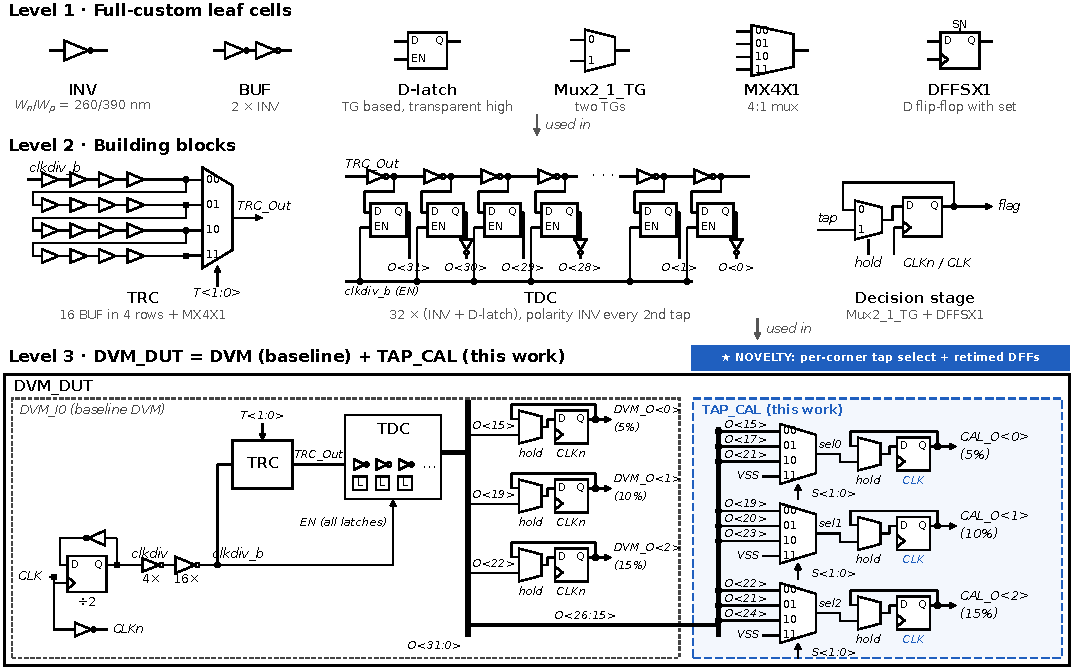
\includegraphics[width=\textwidth]{fig_hierarchy}
\caption{Design hierarchy: full-custom leaf cells (top), building blocks (middle), and the device-under-test cell \sig{DVM\_DUT} (bottom), which holds the baseline DVM (\sig{DVM\_I0}) and the added TAP\_CAL block (blue: this work). The DVM and its layout are unchanged; TAP\_CAL reads the TDC taps \sig{O<26:15>}.}
\label{fig:hier}
\end{figure*}

Fig.~\ref{fig:hier} shows the design from the leaf cells up to the DVM and TAP\_CAL.
\begin{itemize}
\item A D flip-flop (DFF) with an inverter from Q back to D divides \sig{CLK} by two, and an inverter makes \sig{CLKn} for the decision stages; a 4$\times$ and a 16$\times$ inverter buffer drive \sig{clkdiv\_b} to the TRC and to all 32 latch clocks.
\item The TRC is 16 buffers and a 4:1 mux (\sig{MX4X1}) selected by $T\langle1{:}0\rangle$.
\item The TDC is 32 inverters with a transparent-high latch on each tap (\sig{O<31>} first, \sig{O<0>} last) and a polarity inverter after every second latch, so reached taps read 0.
\item While \sig{clkdiv\_b} is high, the edge travels down the chain; when it falls, the latches hold a thermometer code. A droop slows TRC and TDC alike, so fewer stages are reached.
\item Decision stage (baseline): a transmission-gate (TG) mux passes one tap during the hold phase (else recirculates its own output) into a DFF clocked on the falling \sig{CLK} edge, giving \sig{DVM\_O<2:0>}.
\end{itemize}





\begin{figure*}[!t]
\centering
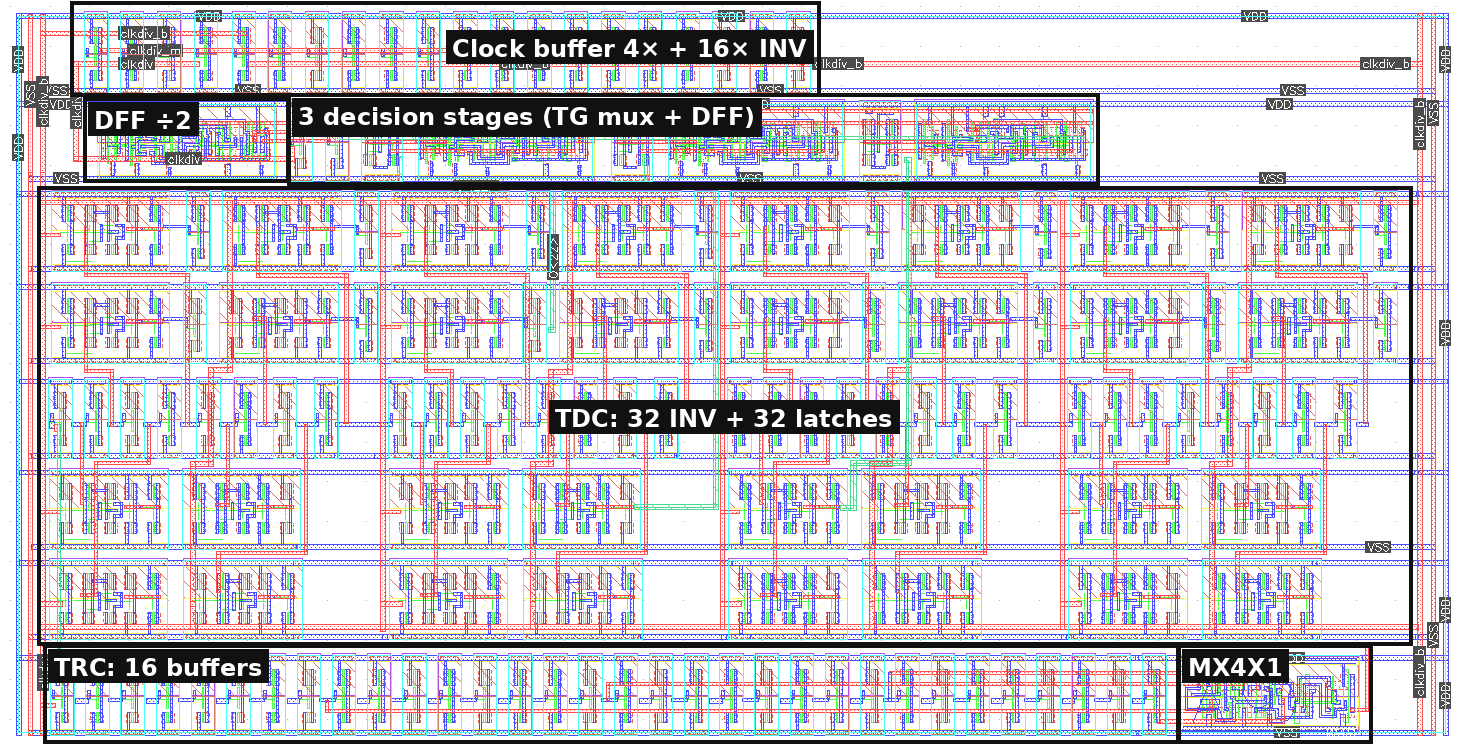
\includegraphics[width=\textwidth]{img_dvm_layout_annot}\\[1pt]
\footnotesize (a) DVM, $36.17\times18.21~\mu$m$^2$ = 658.7~$\mu$m$^2$, with the main blocks marked\\[6pt]
\begin{minipage}[c]{0.42\textwidth}\centering
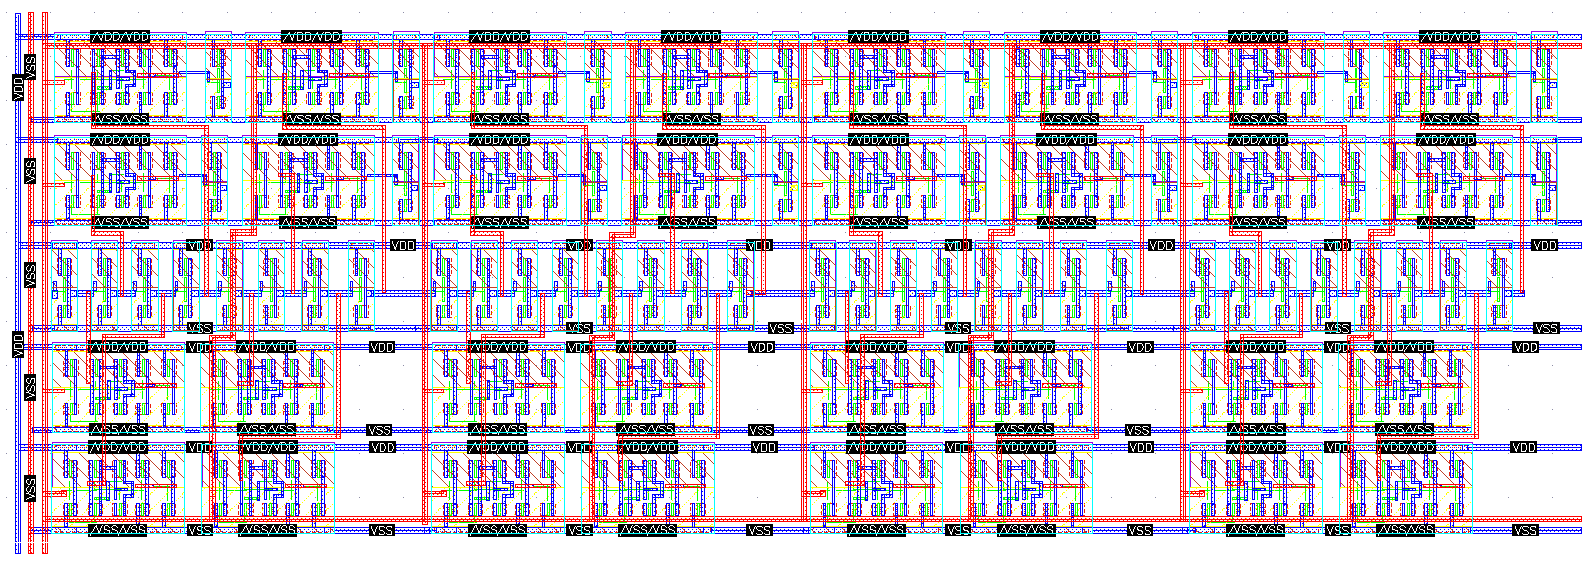
\includegraphics[width=\linewidth]{img_tdc_layout_c}\\[0pt]
\footnotesize (b) TDC (32 inverters + 32 latches)
\end{minipage}\hspace{0.04\textwidth}
\begin{minipage}[c]{0.40\textwidth}\centering
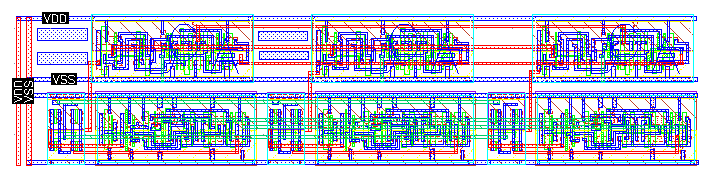
\includegraphics[width=0.8\linewidth]{img_tapcal_layout_c}\\[0pt]
\footnotesize (c) TAP\_CAL\\[6pt]
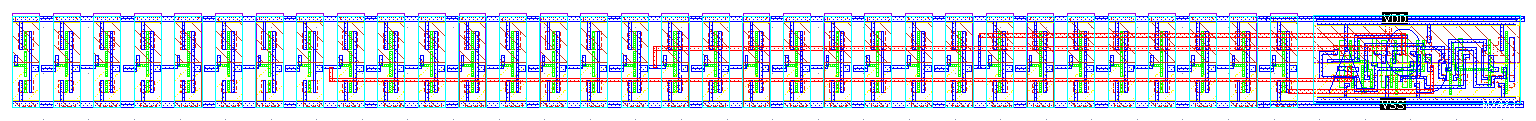
\includegraphics[width=\linewidth]{img_trc_layout_c}\\[0pt]
\footnotesize (d) TRC (16 buffers + \sig{MX4X1})
\end{minipage}\\[6pt]
\begin{tabular}{@{}c@{\hspace{12pt}}c@{\hspace{12pt}}c@{\hspace{12pt}}c@{\hspace{12pt}}c@{}}
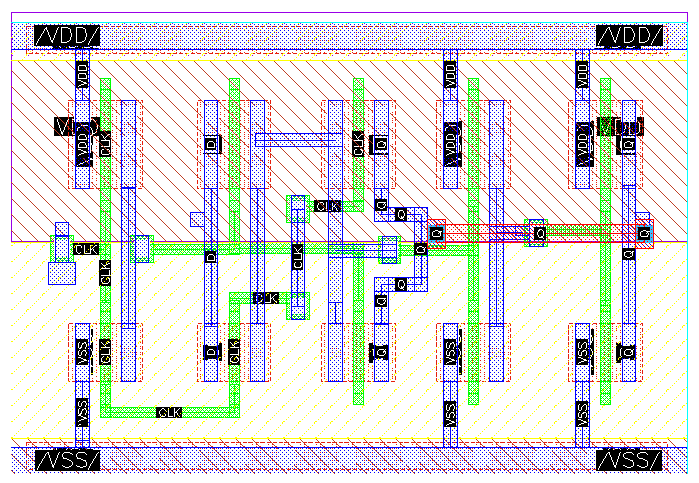
\includegraphics[height=0.115\textwidth]{img_latch_layout_c} &
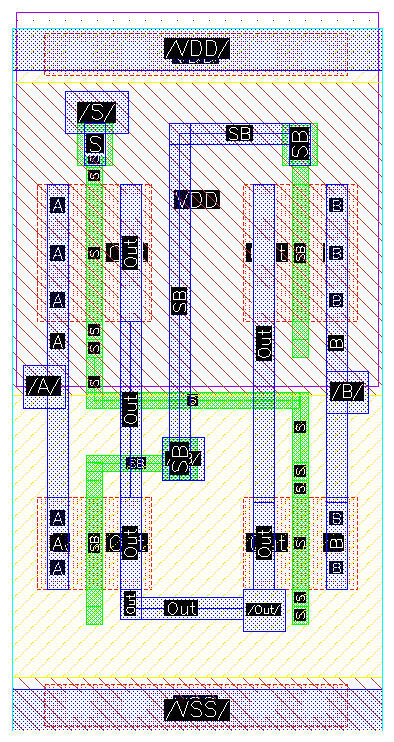
\includegraphics[height=0.115\textwidth]{img_mux2_layout_c} &
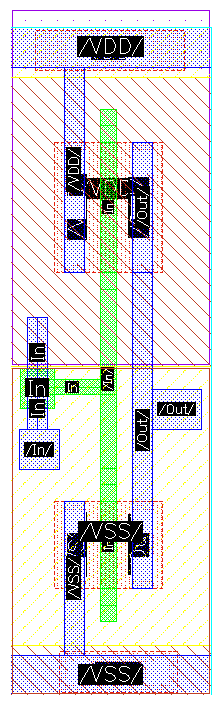
\includegraphics[height=0.115\textwidth]{img_inv_layout_c} &
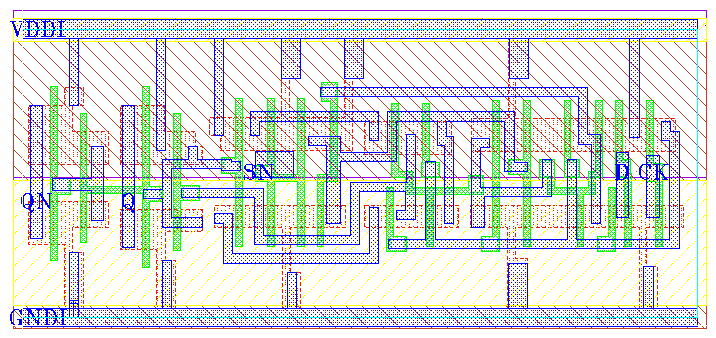
\includegraphics[height=0.115\textwidth]{img_dff_layout_c} &
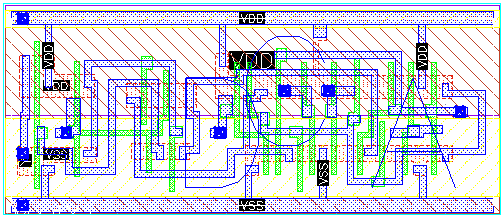
\includegraphics[height=0.115\textwidth]{img_mux4_layout_c} \\
\footnotesize (e) D-latch & \footnotesize (f) TG mux & \footnotesize (g) Inverter & \footnotesize (h) DFF & \footnotesize (i) 4:1 mux (\sig{MX4X1})
\end{tabular}
\caption{Layouts (DRC clean, LVS matched). (a) Full DVM; (b)--(i) building blocks and leaf cells, not to the same scale.}
\label{fig:impl}
\end{figure*}

\subsection{Design Equations}
With clock period $t_{clk}$, sampling window $T_w = t_{clk}$ (half the \sig{clkdiv} period), TRC delay $t_{TRC}$, stage delay $t_s$ and $N$ the number of stages the edge reaches:
\begin{equation}
\mathrm{code} = \left\lfloor (T_w - t_{TRC})/t_s \right\rfloor, \qquad T_w = t_{TRC} + N t_s .
\label{eq:code}
\end{equation}
Gate delay follows the alpha-power law~\cite{sakurai}, $t_s \propto C_L V_{DD}/(V_{DD}-V_t)^{\alpha}$, with load capacitance $C_L$, threshold voltage $V_t$ and velocity-saturation index $\alpha$ ($1<\alpha\le2$). A droop that slows TRC and TDC by the fraction $\delta$ shifts the code by
\begin{equation}
\Delta\mathrm{code} \approx -\,\delta\,T_w/t_s .
\label{eq:shift}
\end{equation}
The code is read from the transistor-level latch outputs in the hold phase (reached taps read 0):
\begin{equation}
\mathrm{code} = 32 - \textstyle\sum_{k=0}^{31} O_k(t_h)/V_{DD},
\label{eq:sum}
\end{equation}
with $O_k$ the voltage of tap \sig{O<k>} and $t_h$ inside the hold phase (10~ns without droop, 20~ns at the droop bottom). Tap \sig{O<k>} is unreached, and its flag fires, when
\begin{equation}
\mathrm{flag}_k = 1 \iff \mathrm{code} \le 31-k .
\label{eq:flag}
\end{equation}
Resolution is set by the loading factor $\kappa = t_s/\tau_{FO1}$, where $\tau_{FO1}$ is the delay of an inverter driving one identical inverter (fan-out of one, FO1). With $P_{act}$ the average active power, the energy per clock cycle is $E_{cyc} = P_{act}\cdot t_{clk}$ (one decision every two cycles).

\begin{figure*}[!t]
\centering
\begin{tabular}{@{}c@{\hspace{12pt}}c@{}}
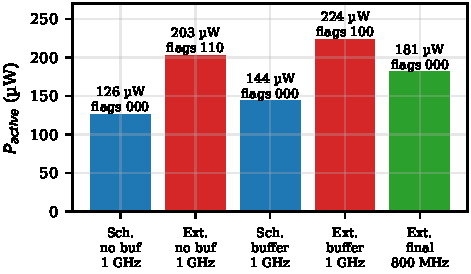
\includegraphics[width=0.40\textwidth]{fig_prepost} &
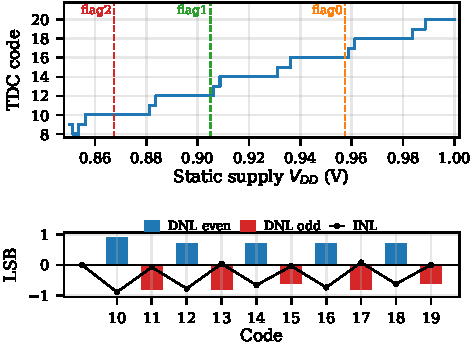
\includegraphics[width=0.40\textwidth]{fig_static} \\[-2pt]
\footnotesize (a) Power and flags through the fixes & \footnotesize (b) Code vs.\ static supply
\end{tabular}
\caption{DVM at TT, 27~$^\circ$C. (a) Active power and no-droop flags \sig{DVM\_O<0:2>} through the design steps: schematic (Sch.) and extracted (Ext.) at the original 1~GHz, without and with the clock buffer, and the final 800~MHz design; red: false flags, green: final. (b) Final post-layout design, 800~MHz: code vs.\ static supply (2.5-mV sweep; dashed: supply at which each flag switches) and DNL/INL per code.}
\label{fig:post}
\end{figure*}

\subsection{Improvement: TAP\_CAL}
Process and temperature shift the no-droop code (9 to 28 across corners, even with the $T$ trim) far more than a 15\% droop does (11 codes), so fixed taps false-alarm at slow corners. TAP\_CAL (Fig.~\ref{fig:hier}, bottom right) is a separate block that reads \sig{O<26:15>}. Per flag, a 4:1 mux selects one of four taps with $S\langle1{:}0\rangle$, chosen per die from the no-droop code (Table~\ref{tab:tap}), so the thresholds follow the die. The selected tap goes through a copy of the decision stage.

The decision DFFs are \emph{retimed} to the rising \sig{CLK} edge, i.e.\ the end of the hold phase. In the baseline the falling edge samples 625~ps after \sig{CLK} rises, but latch close plus clock path takes 317~ps at TT, 27~$^\circ$C and over 500~ps at the slow-slow (ss) corner, 125~$^\circ$C (divider clock-to-Q plus buffer; Section~\ref{sec:pvt}). Adding mux and setup times leaves no margin there. With $S=11$ (inputs tied low) the baseline-timed DFFs still output 111, i.e.\ they never loaded; after retiming they output 000. $S=11$ disables the flags where the TDC is out of range.

\begin{table}[!t]
\caption{TAP\_CAL Tap Selection (Flag Fires When Code $\le 31-k$)}
\label{tab:tap}
\centering\footnotesize
\setlength{\tabcolsep}{3pt}
\begin{tabular}{cccccl}
\toprule
$S$ & No-droop code & 5\% & 10\% & 15\% & Used at \\
\midrule
00 & $\approx$20 & \sig{O<15>} & \sig{O<19>} & \sig{O<22>} & 27~$^\circ$C, cold (with $T$) \\
01 & $\approx$16 & \sig{O<17>} & \sig{O<20>} & \sig{O<21>} & ff, 125~$^\circ$C \\
10 & 12--14 & \sig{O<21>} & \sig{O<23>} & \sig{O<24>} & tt/fs/sf 125, ss 27 \\
11 & 9 (aliased) & 0 & 0 & 0 & ss 125 (disabled) \\
\bottomrule
\end{tabular}
\end{table}

% =====================================================================
\begin{figure*}[!t]
\centering
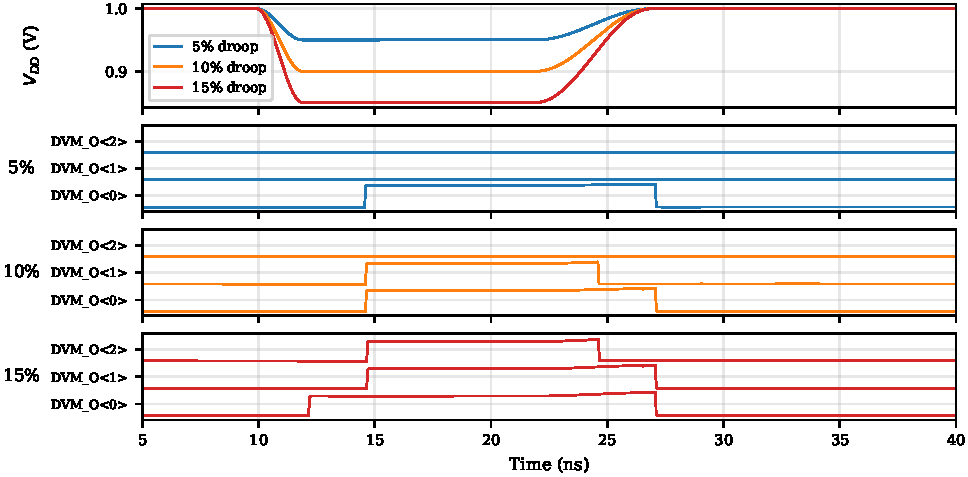
\includegraphics[width=0.9\textwidth]{fig_w1}
\caption{Post-layout 5/10/15\% droops (TT, 27~$^\circ$C): supply and the transistor-level decision outputs \sig{DVM\_O<0:2>} for each droop depth.}
\label{fig:w1}
\end{figure*}

\begin{figure}[!t]
\centering
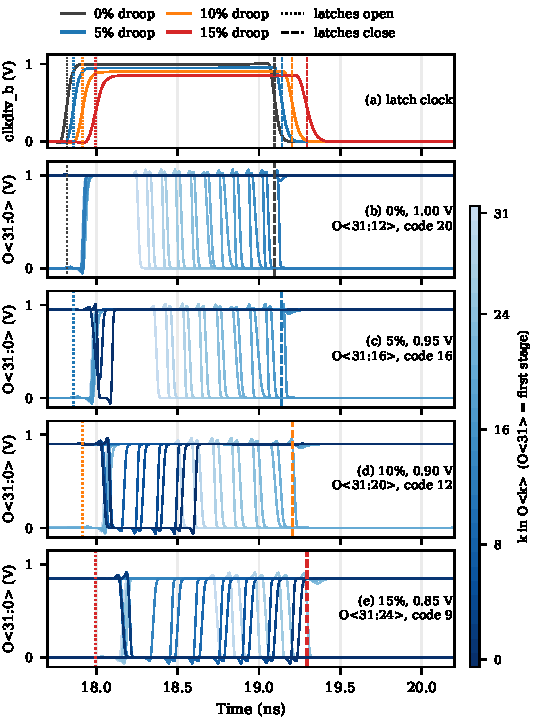
\includegraphics[width=\columnwidth]{fig_tdc_droop}
\caption{TDC taps in one sampling window at the droop bottom (TT, 27~$^\circ$C, 800~MHz). (a) Latch clock \sig{clkdiv\_b} for each droop; dotted: latches open, dashed: latches close. (b)--(e) All 32 taps \sig{O<31:0>} at 0/5/10/15\% droop, coloured from \sig{O<31>} (first stage, light) to \sig{O<0>} (dark); labels give $V_{DD}$, the held reached taps and the code. The taps reset to 1 when the latches open and fall one by one; the deeper the droop, the fewer fall before the latches close. At 10\% and 15\% the dark traces near the window start are edges of the previous window still in the last stages; at 15\% \sig{O<0>} is held at 0, a one-LSB bubble.}
\label{fig:taps}
\end{figure}

\section{Implementation}\label{sec:impl}
All cells are full custom: $L=45$~nm, $W_n/W_p=260/390$~nm (mux 145/215~nm), 2-$\mu$m rows, Metal1 rails, Metal2 buses. The DVM is $36.17\times18.21~\mu$m$^2$ (Fig.~\ref{fig:impl}a), DRC clean, LVS matched and parasitic (RC) extracted. TAP\_CAL is also laid out (Fig.~\ref{fig:impl}c), LVS matched and extracted. The final top cell \sig{DVM\_TOP} holds only the device-under-test (DUT) cell \sig{DVM\_DUT} (DVM + TAP\_CAL, Fig.~\ref{fig:hier}) and the test bench \sig{DVM\_TB} (Verilog-A droop source, the only behavioural block, a 0-V supply probe and the clock, reset and select sources); a \sig{config} view binds both blocks to their extracted views. Eight saved ADE~L states on this cell (Appendix~A) reproduce the post-layout and worst-corner values of the figure-of-merit (FoM) summary in Section~\ref{sec:summary}, except the corner-sweep false-warning counts and the TAP\_CAL power overhead (the pre-layout and Monte Carlo columns come from the schematic); the DVM power is read from its own supply terminal. The earlier corner sweep (Section~\ref{sec:pvt}), droop trains and detection map were run in ADE~XL with the TAP\_CAL schematic. All codes, flags, latencies and powers are measured on transistor-level nets, using \eqref{eq:sum} for the code.





% =====================================================================
\section{Results and Discussion}\label{sec:results}
The metrics follow the objectives: the code and its voltage sensitivity (resolution), correct flags and false warnings (O1, O2), latency from the droop to the flag (O3), power, energy and area (O4), and their spread over PVT corners and Monte Carlo (MC) samples (O6). Unless stated, results are post-layout at the typical corner (TT), 27~$^\circ$C.
\subsection{Unit Cells and Pre- vs.\ Post-Layout}



Table~\ref{tab:unit} lists the measured cell delays. A stand-alone TDC reaches 7/11/15 stages for 200/300/400-ps windows (25.0~ps/stage). Its $\kappa=3.0$ is above the 1.4 of~\cite{bowman_tcas} because each chain inverter also drives a latch TG. Extraction makes the stage 1.75$\times$ slower but the FO1 inverter only 1.29$\times$ (10.78~ps) and a buffer 1.37$\times$ (25.2~ps), so most of the loss is the wiring between TDC stages ($\kappa$: 3.0$\to$4.4). At the same 800~MHz, $T{=}00$ and TT, extraction raises $t_{TRC}$ from 175.9 to 325.6~ps and the clock path from 155 to 317~ps; the schematic code saturates at 32, the extracted one reads 20. The first post-layout run kept the schematic design point (1~GHz, no clock buffer) and raised two false flags. Table~\ref{tab:base} and Fig.~\ref{fig:post}a show the recovery.

\begin{table}[!t]
\caption{Cell Delays ($V_{DD}=1.0$~V, TT, 27~$^\circ$C)}
\label{tab:unit}
\centering\footnotesize
\setlength{\tabcolsep}{3pt}
\begin{tabular}{lccc}
\toprule
Metric & \cite{bowman_tcas} & Schematic & Extracted \\
\midrule
$\tau_{FO1}$ & $\approx$4.6~ps$^\S$ & 8.33~ps & 10.78~ps \\
Buffer (FO1) & -- & 18.34~ps & 25.2~ps \\
$\div$2 DFF clock-to-Q & -- & 49.28~ps & 192.6~ps (loaded) \\
TDC stage $t_s$ & 6.5~ps & 25.0 / 26.9~ps$^\ddagger$ & 47.1~ps \\
$\kappa=t_s/\tau_{FO1}$ & 1.4 & 3.0 & 4.4 \\
\bottomrule
\multicolumn{4}{l}{$^\ddagger$stand-alone TDC / inside the DVM.}\\
\multicolumn{4}{l}{$^\S$derived: \cite{bowman_tcas} gives $t_s=6.5$~ps $=1.4\,\tau_{FO1}$.}
\end{tabular}
\end{table}

\begin{table}[!t]
\caption{Post-Layout Fix of the Direct Implementation (TT, 27~$^\circ$C)}
\label{tab:base}
\centering\footnotesize
\setlength{\tabcolsep}{3pt}
\begin{tabular}{lcc}
\toprule
Metric & 1~GHz, no buffer & 800~MHz, buffered \\
\midrule
False flags & 2 of 3 & 0 of 3 \\
Latch-clock edge & triangular & 65~ps rise \\
Droop levels flagged & 0 of 3 & 3 of 3 \\
$P_{act}$ (probe)$^\ast$ & 203~$\mu$W & 181~$\mu$W \\
\bottomrule
\multicolumn{3}{p{0.9\columnwidth}}{$^\ast$Earlier 0-V probe measurement (DVM + test-bench clock path); the final DVM-only value is 138.4~$\mu$W (Section~\ref{sec:transfer}).}\\
\end{tabular}
\end{table}



\begin{figure*}[!t]
\centering
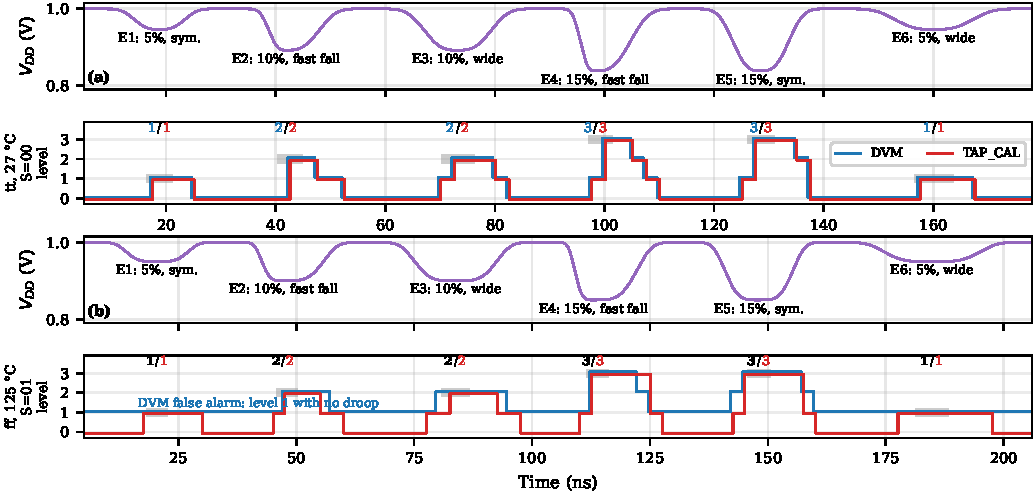
\includegraphics[width=\textwidth]{fig_train.pdf}
\caption{Droop train (post-layout, 800~MHz, $T{=}00$). (a) TT, 27~$^\circ$C, $S{=}00$; (b) ff, 125~$^\circ$C, $S{=}01$, exact depths. Level (0--3) of the DVM (blue) and TAP\_CAL (red); gray bars: expected level. Labels: DVM/TAP\_CAL level reached (bold black: wrong).}
\label{fig:train}
\end{figure*}

\subsection{Transfer Curve, Waveforms, Latency and Power}\label{sec:transfer}
A 2.5-mV static sweep (Fig.~\ref{fig:post}b) gives 13.3~mV per least significant bit (LSB) on average between 0.856 and 0.989~V. Even codes are 22.5~mV wide and odd codes 2.5--5~mV, because the edge crosses alternate stages as rising and falling transitions and the taps are 28 and 60~ps apart; the differential nonlinearity (DNL) is $-$0.81 to $+$0.89~LSB and the integral nonlinearity (INL) $-$0.89 to $+$0.08~LSB (endpoint fit, sweep step 0.19~LSB). The flags switch at 0.9575, 0.905 and 0.8675~V, i.e.\ at 4.25, 9.5 and 13.25\% droop, each just before its nominal level. Below 0.856~V the code aliases. Fig.~\ref{fig:w1} and Table~\ref{tab:droop} show the dynamic response and Fig.~\ref{fig:taps} the taps at the droop bottom. In the final bench the DVM draws 138.4~$\mu$W from its supply terminal (173~fJ per clock cycle). The energy the DVM uses from the droop onset until \sig{DVM\_O<0>} rises is 627, 706 and 280~fJ for 5, 10 and 15\% droops. With the clock stopped, leakage is 5.67~nW (6.67~nW with TAP\_CAL), rising to 90.2~nW (112~nW) at ff, 125~$^\circ$C.







\begin{table}[!t]
\caption{Post-Layout Droop Response (TT, 27~$^\circ$C, 800~MHz)}
\label{tab:droop}
\centering\footnotesize
\setlength{\tabcolsep}{2pt}
\begin{tabular}{lccc}
\toprule
Droop & 5\% & 10\% & 15\% \\
\midrule
Code & 20$\rightarrow$16 & 20$\rightarrow$12 & 20$\rightarrow$9 \\
\sig{DVM\_O<0:2>} & 100 & 110 & 111 \\
Latency flag0/1/2 (ns) & 4.10/--/-- & 4.31/4.31/-- & 1.95/4.45/4.45 \\
Flags cleared (ns) & 27.09 & 27.09 & 27.09 \\
Shortest flagged (FWHM)$^a$ & 2~ns & 1~ns$^b$ & 1~ns$^b$ \\
\bottomrule
\multicolumn{4}{p{0.95\columnwidth}}{$^a$V-shaped droop, best of two sampling phases. $^b$Graded one level low.} \\
\end{tabular}
\end{table}

\subsection{Droop Train}
Fig.~\ref{fig:train} applies six smooth droops of different depth and shape in one post-layout run. Each droop has a rounded bottom held near its depth for 4.5--7~ns.
\begin{itemize}
\item \textbf{TT, 27~$^\circ$C} (a; droops overshoot their nominal depth by up to 8\%, less than one code): DVM and TAP\_CAL grade all six events correctly. The level is flagged 0.5--2.7~ns after the supply reaches it (TAP\_CAL +0.5~ns).
\item \textbf{ff, 125~$^\circ$C} (b; exact depths): the DVM 5\% flag never clears, so 5\% droops are invisible. TAP\_CAL has no false alarm and grades all six events correctly.
\end{itemize}



\subsection{Detection Map}
Fig.~\ref{fig:matrix} sweeps Gaussian droop depth (2.5--15\%) and width (full width at half maximum, FWHM, 1--12~ns) in one post-layout run at TT, 27~$^\circ$C (40 droops). There are no false flags, and 2.5\% is never flagged. From 8~ns every droop is graded correctly by both the DVM and TAP\_CAL. From 4~ns every droop $\ge$5\% is detected, but 10\% and 15\% read one level low: the thresholds sit on the nominal codes, so the full depth must last a whole measurement ($\approx$1.3~ns, every 2.5~ns). At 1--2~ns detection depends on where the droop falls relative to the sampling clock.

\begin{figure}[!t]
\centering
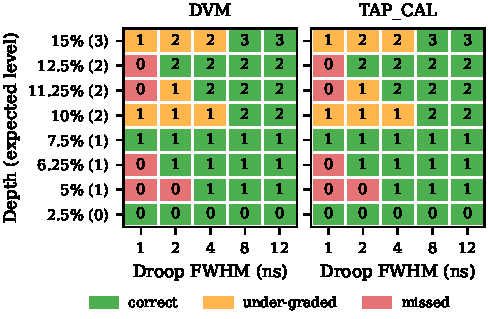
\includegraphics[width=\columnwidth]{fig_matrix.pdf}
\caption{Detection map (post-layout, TT, 27~$^\circ$C, $T{=}S{=}00$): flag level reached by 40 Gaussian droops of different depth and width.}
\label{fig:matrix}
\end{figure}

\begin{figure*}[!t]
\centering
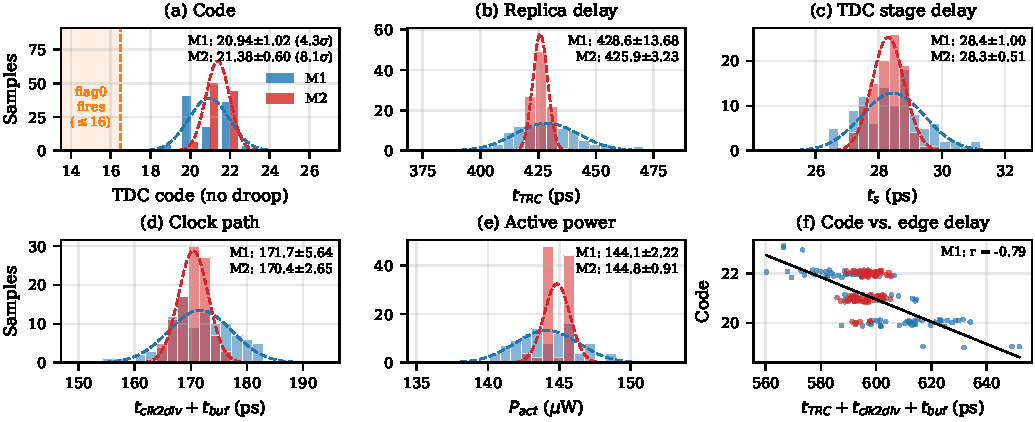
\includegraphics[width=\textwidth]{fig_mc.pdf}
\caption{Monte Carlo distributions (schematic, 100 samples, 1~GHz, $T{=}11$, TT, 27~$^\circ$C, no droop). (a) TDC code with the flag0 region; (b) replica delay; (c) TDC stage delay; (d) clock path; (e) active power; (f) code vs.\ edge delay. Dashed: fitted normal.}
\label{fig:mc}
\end{figure*}



\subsection{PVT Corners}\label{sec:pvt}
The 15 corners combine the typical (tt), slow (ss), fast (ff) and mixed (fs, sf) NMOS/PMOS models with $-40$, 27 and 125~$^\circ$C. Table~\ref{tab:cal} lists the no-droop code at each, with the TRC trim $T$ set per corner. Temperature matters as much as process: tt moves from 20 at 27~$^\circ$C to 12 at 125~$^\circ$C, while process spreads the 125~$^\circ$C code from 9 (ss) to 16 (ff); fs/sf track tt.
\begin{itemize}
\item \textbf{Fastest corner, ff $-40~^\circ$C:} code 28 even with maximum trim ($T{=}11$), so a 5\% droop (code 22) stays above the threshold.
\item \textbf{Slowest corner, ss 125~$^\circ$C:} code 9; the TDC is out of range.
\end{itemize}
\begin{table}[!t]
\caption{Baseline vs.\ TAP\_CAL Flags (0/5/10/15\% Droop)}
\label{tab:cal}
\centering\footnotesize
\setlength{\tabcolsep}{2pt}
\begin{tabular}{lcccc}
\toprule
Corner ($^\circ$C) & $S$/$T$ & Code & \sig{DVM\_O} & \sig{CAL\_O} \\
\midrule
tt 27 & 00/00 & 20 & 000/100/110/111 & 000/100/110/111 \\
fs 27 & 00/00 & 20 & 000/100/110/111 & 000/100/110/111 \\
sf 27 & 00/00 & 20 & 000/100/110/111 & 000/100/110/111 \\
ff 27 & 00/10 & 20 & 000/100/110/111 & 000/100/110/111 \\
ss 27 & 10/00 & 14 & \textbf{100}/\textbf{110}/\textbf{111}/111 & 000/100/\textbf{111}/111 \\
\midrule
tt $-40$ & 00/11 & 18 & 000/100/110/111 & 000/100/110/111 \\
fs $-40$ & 00/11 & 18 & 000/100/110/111 & 000/100/110/111 \\
sf $-40$ & 00/11 & 18 & 000/100/110/111 & 000/100/110/111 \\
ff $-40$ & 00/11 & 28 & 000/\textbf{000}/\textbf{000}/\textbf{110} & 000/\textbf{000}/\textbf{000}/\textbf{110} \\
ss $-40$ & 00/00 & 20 & 000/100/110/111 & 000/100/110/111 \\
\midrule
tt 125 & 10/00 & 12 & \textbf{110}/\textbf{111}/\textbf{111}/111 & 000/100/\textbf{111}/111 \\
fs 125 & 10/00 & 12 & \textbf{110}/\textbf{111}/\textbf{111}/111 & 000/100/\textbf{111}/111 \\
sf 125 & 10/00 & 12 & \textbf{110}/\textbf{111}/\textbf{111}/111 & 000/100/\textbf{111}/111 \\
ff 125 & 01/00 & 16 & \textbf{100}/100/110/111 & 000/100/110/111 \\
ss 125 & 11/00 & 9 & \textbf{111}/\textbf{111}/\textbf{111}/111 & 000/\textbf{000}/\textbf{000}/\textbf{000} \\
\midrule
\multicolumn{3}{l}{Detected correctly} & 41/60 & 50/60 \\
\multicolumn{3}{l}{False warnings} & 16/60 & 4/60 \\
\bottomrule
\multicolumn{5}{p{0.95\columnwidth}}{60 cases: 15 corners $\times$ 4 droop levels; expected 000/100/110/111. Bold: wrong. False warning: flag level above the applied droop.}
\end{tabular}
\end{table}

\begin{table}[!t]
\caption{Monte Carlo (Schematic, 100 Samples, No Droop)}
\label{tab:mc}
\centering\footnotesize
\setlength{\tabcolsep}{3pt}
\begin{tabular}{lcc}
\toprule
$\mu\pm\sigma$ & Process + mismatch & Mismatch only \\
\midrule
Code (range) & $20.9\pm1.0$ (19--23) & $21.4\pm0.6$ (20--22) \\
$t_{TRC}$ (ps) & $428.6\pm13.7$ & $425.9\pm3.2$ \\
$t_s$ (ps) & $28.45\pm1.00$ & $28.29\pm0.51$ \\
$t_{clk2div}+t_{buf}$ (ps) & $171.7\pm5.6$ & $170.4\pm2.6$ \\
$P_{act}$ ($\mu$W) & $144.1\pm2.2$ & $144.8\pm0.9$ \\
Highest flag level & 5.7~mV & 4.9~mV \\
Samples with no false flag & 100/100 & 100/100 \\
Margin to flag0 & $4.3\sigma$ & $8.1\sigma$ \\
\midrule
\multicolumn{3}{l}{Global share of variance: $t_{TRC}$ 94\%, $t_s$ 74\%, code 66\%, $P$ 83\%} \\
\bottomrule
\end{tabular}
\end{table}

With fixed taps the DVM grades only 41 of the 60 corner--droop cases correctly. The TRC trim lowers the code at fast and cold corners but cannot raise it. At hot corners the TDC runs out of range under droop: the code at the droop bottom stops falling after 5\% and then wraps upward through aliasing (tt 125~$^\circ$C: 12$\rightarrow$10$\rightarrow$12$\rightarrow$17 for 0/5/10/15\%), so 10\% and 15\% cannot be graded there. The slower clock path at these corners (divider clock-to-Q plus buffer: 416~ps at tt 125~$^\circ$C, 522~ps at ss 125~$^\circ$C, vs.\ 317~ps at TT) and the longer stage (65--81~ps vs.\ 47.1~ps) both shrink the usable window.

\begin{table*}[!t]
\caption{Figure-of-Merit Summary}
\label{tab:fom}
\centering\footnotesize
\setlength{\tabcolsep}{3.1pt}
\begin{tabular}{llccccc}
\toprule
FoM & Condition & Spec & \makecell{Pre-layout\\(1~GHz)} & \makecell{Post-layout\\(800~MHz)} & \makecell{Worst corner} & \makecell{Monte Carlo} \\
\midrule
Resolution & mV/LSB, static sweep & -- & 10~mV & 13.3~mV & 25~mV (125~$^\circ$C) & n/m \\
DNL / INL (LSB) & codes 10--19 & -- & n/m & $-$0.81..0.89 / $-$0.89..0.08 & n/m & n/m \\
Detection levels & flags & 5/10/15\% & 5/10/15\%$^\dagger$ & 5/10/15\% & 5\% only (hot) & -- \\
Flag switching & static $V_{DD}$ & 0.95/0.90/0.85~V & n/m & 0.958/0.905/0.868~V & n/m & n/m \\
Shortest flagged droop & FWHM, 5\% / 10\% & -- & n/m & 2 / 1~ns & n/m & n/a \\
Detection latency & droop$\rightarrow$flag & $\le$5~ns & 3.31~ns & 1.9--4.5~ns & 4.94~ns$^\S$ & n/a \\
False warnings, no droop & 15 corners & 0 & n/m & DVM 6/15; TAP\_CAL 0/15 & ss 27: 100 / CAL 000 & 0/100 \\
Active power & at $f_{max}$ & $\le$300~$\mu$W & 143.9~$\mu$W & 138.4~$\mu$W & 202.3~$\mu$W & $144.1\pm2.2~\mu$W$^\ddagger$ \\
TAP\_CAL power overhead & TT, no droop & -- & n/a & $\approx$11~$\mu$W (6\%) & n/m & n/a \\
Energy / cycle & $P/f$ & -- & 144~fJ & 173~fJ & 253~fJ & $144\pm2$~fJ$^\ddagger$ \\
Energy / detection $E_{tot}$ & $\int P\,dt$ to flag & -- & n/m & 0.28--0.71~pJ & 0.65~pJ & n/a \\
RWP & (mV/LSB)$\times T_w$ & -- & 10~mV$\cdot$ns & 16.6~mV$\cdot$ns & n/m & n/a \\
ERP & $(P/f)\times$(mV/LSB) & -- & 1.44~pJ$\cdot$mV & 2.29~pJ$\cdot$mV & n/m & n/a \\
FoM1 = RWP$\times$ERP & lower is better & -- & 1.44$\times10^4$ & 3.80$\times10^4$ & n/m & n/a \\
FoM2 = FoM1$\times$Area & lower is better & -- & n/a & 2.50$\times10^7$ & n/a & n/a \\
Leakage & clock stopped & -- & n/m & 5.67 (6.67)~nW$^\ast$ & 90.2 (112)~nW$^\ast$ & n/a \\
Area & layout (DVM) & $\le$0.005~mm$^2$ & n/a & 658.7~$\mu$m$^2$ & n/a & n/a \\
Calibration points & per die & -- & -- & 1 (sets $S$, $T$) & -- & -- \\
Reference; Verilog-A & -- & -- & -- & clock only; none$^\P$ & -- & -- \\
\bottomrule
\multicolumn{7}{p{0.97\textwidth}}{$^\dagger$Same taps \sig{O<15>/<19>/<22>} in the schematic; not re-simulated with droops before layout. $^\ddagger$Schematic, 1~GHz, $T{=}11$. $^\S$TAP\_CAL, ss, 27~$^\circ$C, 10\% droop. Worst-corner power and energy: ff, $-40~^\circ$C; leakage: ff, 125~$^\circ$C. $^\P$Only the droop source in the test bench is Verilog-A. RWP: resolution--window product; ERP: energy--resolution product; RWP, ERP, FoM1, FoM2 in the course units (mV, ns, fJ, $\mu$m$^2$); $T_w = t_{clk}$. $^\ast$In brackets: with TAP\_CAL. Post-layout and worst-corner values from the saved ADE~L states (Appendix~A). n/m: not measured; n/a: not applicable.}
\end{tabular}
\end{table*}

\begin{table*}[!t]
\caption{Comparison With Published Supply-Droop Monitors}
\label{tab:comp}
\centering\scriptsize
\setlength{\tabcolsep}{2pt}
\begin{tabular}{>{\raggedright\arraybackslash}p{2.2cm}*{8}{>{\centering\arraybackslash}p{1.78cm}}}
\toprule
 & \cite{muhtaroglu} & \cite{bowman_cicc,bowman_tcas} & \cite{whatmough_jssc} & \cite{mizrahi} & \cite{shifman} & \cite{du_tcas} & \cite{qian_iscas} & \textbf{This work} \\
\midrule
Published & JSSC'04 & CICC'10 / TCAS-I'11 & JSSC'17 & Access'21 & JSSC'22 & TCAS-I'23 & ISCAS'25 & Course project \\
Technology & 90~nm & 45~nm & 28~nm & 65~nm & 65~nm & 28~nm & 22~nm & 45~nm \\
Principle & analog sensing & TRC + TDC & digital delay sensor & CCO + counter & inverter / cap.\ ratio & ring osc.\ + Nyquist ctr. & multi-phase ring-osc.\ TDC & TRC + latch TDC \\
All-digital & no & yes & yes & no & no & yes & yes & yes \\
Sampling rate & core clock & 1 per 2 clk & 0.4--2.24~GS/s & 1.6-$\mu$s count & 500~MHz & 0.5--2~GS/s & 2~GS/s & 400~MS/s \\
Resolution & 20~mV step (7~mV hi-res) & 6.5-ps TDC step & 3.3~mV @ 0.8~GS/s & 10~mV & 0.9\%~$V_{DD}$ & 1.92--7.32~mV/LSB & 7.01~mV/LSB & 13.3~mV/LSB \\
DNL / INL & n/r & n/r & 0.6 / 0.9~LSB & n/r & n/r & n/r & n/r & 0.89 / 0.89~LSB \\
Detection levels & 1 threshold & 3 flags & multi-bit code & multi-bit code & 3 levels & multi-bit code & multi-bit code & 3 levels \\
Detection latency & n/r & 2-cycle readout & 2 cycles & $\approx$5~ns & 2--3.5~ns & 0 (prediction) & n/r & 1.9--4.5~ns \\
Min.\ duration & 100~ps (sim.) & n/r & n/r & n/r & $\approx$2~ns & n/r & n/r & 1~ns FWHM \\
False warnings, corners & n/r & n/r & n/r & n/r & n/r & n/r & n/r & 0/15 \\
Area ($\mu$m$^2$) & n/r & 1990 & 108500$^\ddagger$ & 8800 & 8500 & 1427 & 819 & 659$^\ast$ \\
Power & n/r & n/r & 416~$\mu$W$^\ddagger$ & 297~$\mu$W & 62~$\mu$W & 4.93~mW & 2.19~mW & 138~$\mu$W \\
Energy / cycle & n/r & n/r & 520~fJ$^\dagger$ & n/r & 124~fJ$^\dagger$ & 2.46~pJ$^\dagger$ & 1.10~pJ$^\dagger$ & 173~fJ \\
$E_{tot}$ per detection & n/r & n/r & n/r & n/r & n/r & n/r & n/r & 0.28--0.71~pJ \\
RWP (mV$\cdot$ns) & n/r & n/r & n/r & n/r & n/r & n/r & n/r & 16.6 \\
ERP (pJ$\cdot$mV) & n/r & n/r & n/r & n/r & n/r & n/r & n/r & 2.29 \\
FoM1 & n/r & n/r & n/r & n/r & n/r & n/r & n/r & 3.80$\times10^4$ \\
FoM2 & n/r & n/r & n/r & n/r & n/r & n/r & n/r & 2.50$\times10^7$ \\
Leakage & n/r & n/r & n/r & n/r & n/r & n/r & n/r & 5.7~nW \\
Calibration & 5-bit DAC per module & $V$/$f$ sweep & $V$ sweep (LUT) & 2 temperatures & 1 temperature & $V$ sweep, 16 temps. & n/r & 1 point \\
Reference required & quiet supply + current ref. & clock & clock & analog bias, quiet supply & quiet analog supply & clock + temp.\ sensor & clock (multi-phase) & clock only \\
PVT handling & DAC calibration & TRC calibration & software F-to-V & DC-level indep. & cap.\ ratio & dynamic PVT cal. & n/r & $T$ trim + TAP\_CAL \\
Verilog-A blocks & n/a (silicon) & n/a (silicon) & n/a (silicon) & n/a (silicon) & n/a (silicon) & n/a (silicon) & n/r & none$^\S$ \\
Result type & measured & measured & measured & measured & measured & measured & simulated & post-layout sim. \\
\bottomrule
\multicolumn{9}{p{0.97\textwidth}}{$^\ast$DVM only; TAP\_CAL not included. $^\S$Only the test-bench droop source is Verilog-A. $^\dagger$Derived here as power / clock (sampling) frequency: 416~$\mu$W / 0.8~GHz, 62~$\mu$W / 500~MHz, 4.93~mW / 2~GHz, 2.19~mW / 2~GHz. $^\ddagger$Whole monitor macro including event engine and trace memory. \cite{shifman}: 62~$\mu$W and 2~ns at 1.2~V, 22~$\mu$W and 3.5~ns at 1.0~V. \cite{du_tcas}: 0 cycles with prediction, 3 cycles without; area of the sensor only. \cite{qian_iscas}: 22~nm HSPICE simulation, 2~GHz, 0.9~V.}
\end{tabular}
\end{table*}

\subsection{TAP\_CAL Results}
Table~\ref{tab:cal} compares the baseline flags (\sig{DVM\_O}) with TAP\_CAL (\sig{CAL\_O}) in the same simulations, with $S$ and $T$ set per corner. Over all 60 cases (15 corners $\times$ 4 droop levels), correct detections rise from 41 to 50 and false warnings fall from 16 to 4; no corner raises a flag without a droop. At hot corners the TDC aliases beyond 5\%, so TAP\_CAL flags the droop but over-grades 10\%. ss 125~$^\circ$C is deliberately disabled, and ff $-40~^\circ$C stays at code 28 even with maximum trim, so only 15\% is caught there. End-of-hold sampling adds about 0.47~ns of latency (e.g.\ 4.31$\rightarrow$4.79~ns at 10\%, TT), and TAP\_CAL adds about 11~$\mu$W (192 vs.\ 181~$\mu$W with the same probe, 6\%).







\subsection{Monte Carlo}
Monte Carlo is run on the schematic (100 samples, Latin hypercube sampling, TT, 27~$^\circ$C, no droop) at 1~GHz with $T{=}11$, which places the nominal code (22) inside the TDC range as in the post-layout design (Fig.~\ref{fig:mc}, Table~\ref{tab:mc}). No sample of either run raises a flag (highest flag level 5.7~mV vs.\ the 0.5~V threshold), so all 100 samples pass. The code spans 19--23 with process + mismatch, a $4.3\sigma$ margin to the flag0 threshold, and 20--22 with mismatch only ($8.1\sigma$). The code tracks the total edge delay sample by sample ($r{=}{-}0.79$, Fig.~\ref{fig:mc}f). Global process causes 94\% of the replica-delay variance, 74\% of the stage-delay variance and 66\% of the code variance. Per-die calibration ($T$, $S$), not upsizing~\cite{pelgrom}, addresses the dominant source.





\subsection{Summary and Comparison}\label{sec:summary}
Table~\ref{tab:fom} summarizes the FoMs and Table~\ref{tab:comp} compares with published monitors (``n/r'': not reported). The DVM alone has the smallest area of the compared monitors (659~$\mu$m$^2$ vs.\ 819~$\mu$m$^2$ for~\cite{qian_iscas} at 22~nm) and the second-lowest power and energy per cycle after~\cite{shifman}, and it needs only a clock. Its resolution, however, is 2--7$\times$ coarser than the 22--28-nm GS/s sensors~\cite{whatmough_jssc,du_tcas,qian_iscas}, and its range is limited by the 32-stage TDC. Our results are post-layout simulation, whereas most cited works are silicon measurements.





\subsection{Limitations}
\begin{itemize}
\item At hot corners the TDC floor (code 9--10) limits TAP\_CAL to one level (droop $\ge$5\%); ss 125~$^\circ$C is disabled.
\item ff $-40~^\circ$C stays at code 27--28 even with maximum trim, so 5\% and 10\% are missed.
\item Thresholds sit on the nominal codes: droops shorter than $\approx$8~ns are under-graded by one level (Fig.~\ref{fig:matrix}). Moving each tap one code earlier would add margin.
\item Rising and falling stage delays differ (taps 28/60~ps apart), giving DNL up to $-$0.81~LSB; balancing the inverter $W_p/W_n$ for equal $t_{pLH}$, $t_{pHL}$ would even the steps.
\item The 1.75$\times$ post-layout stage delay forced 800~MHz, raising energy per cycle from 144 to 173~fJ.
\end{itemize}

% =====================================================================
\section{Conclusion and Future Work}\label{sec:concl}
The post-layout DVM flags 5/10/15\% droops within 1.9--4.5~ns in 659~$\mu$m$^2$ at 138~$\mu$W, with no false alarm in 100 schematic-level Monte Carlo samples. Its fixed thresholds, however, false-alarm at 6 of 15 corners because global process and temperature dominate the code. TAP\_CAL adds per-die selectable thresholds and end-of-hold sampling and raises correct detections from 41/60 to 50/60 and cuts false warnings from 16/60 to 4/60, with none at no droop. At TT, 27~$^\circ$C all six objectives are met (O3: at most 4.94~ns even at the worst corner; O4: 659~$\mu$m$^2$, 138~$\mu$W); with TAP\_CAL, O2 holds at all 15 corners, while O1 is only partly met across corners: ff $-40~^\circ$C misses 5\% and 10\%, and hot corners over-grade 10\%. Future work: buffered TAP\_CAL taps, a longer or faster TDC to remove the hot-corner floor, and using the full 32-bit code for closed-loop adaptive clocking.

\section*{Acknowledgment}
The authors thank Prof.~Viveka, the DVLSI 2026 instructor, and the teaching assistants Sisir Mridha and Samudrala Hareesh at IISc for their guidance. An AI assistant (Claude, Anthropic) was used for guidance on simulation planning, result interpretation and report drafting; all design, layout and simulation work was done by the authors.



\bibliographystyle{IEEEtran}
\bibliography{refs}


\section*{Appendix A: Code Snippets}
\subsection*{A1. Verilog-A Droop Source (Single Droop)}
The only behavioural block in the test bench; it drives the DVM supply through a 0-V current probe.
\begin{lstlisting}
module VDD_droop3(vout);
  output vout; electrical vout;
  parameter real vnom=1.0, vdroop=0.1; // V
  parameter real tdelay=9.9n, tdown=2n;
  parameter real twidth=10n, tup=5n;
  real t, x, t1, t2, t3;
  analog begin
    t = $abstime; t1 = tdelay+tdown;
    t2 = t1+twidth; t3 = t2+tup;
    @(timer(tdelay) or timer(t1)
      or timer(t2) or timer(t3));
    if (t <= tdelay) x = 0.0;
    else if (t < t1)
      x = 0.5*(1-cos(`M_PI*(t-tdelay)/tdown));
    else if (t < t2) x = 1.0;          // hold
    else if (t < t3)
      x = 0.5*(1+cos(`M_PI*(t-t2)/tup));
    else x = 0.0;
    if (t >= tdelay && t <= t3)
      $bound_step(min(tdown,tup)/20);
    V(vout) <+ vnom - vdroop*x;
  end
endmodule
\end{lstlisting}

\subsection*{A2. Droop Train (Fig.~\ref{fig:train}b)}
Six rounded droops; each reaches exactly its depth $a_i$ and stays within 1\% of it for 4.5--7~ns. Fall and recovery widths differ.
\begin{lstlisting}
// d_i(t) = a_i*exp(-0.5*x^4),
// x = |t-c_i|/wf_i or /wr_i
analog function real ushape;
  input tt, c, wf, wr; real tt, c, wf, wr, x;
  begin
    x = (tt < c) ? (c-tt)/wf : (tt-c)/wr;
    ushape = (x > 3.0) ? 0.0 : exp(-0.5*x*x*x*x);
  end
endfunction
// a = 5/10/10/15/15/5 %, c = 20.5 ... 184.8 ns
d = a1*ushape(t,c1,wf1,wr1) + ...
  + a6*ushape(t,c6,wf6,wr6);
V(vout) <+ vnom - d;
\end{lstlisting}

\subsection*{A3. Detection Map (Fig.~\ref{fig:matrix})}
Gaussian droops: 8 depths $\times$ 5 widths (\texttt{nw}${}=5$), 8-ns gap.
\begin{lstlisting}
// FWHM 1,2,4,8,12 ns; depth 2.5 ... 15 %
for (i = 0; i < nw; i = i+1) begin
  s = fw(i)/2.3548;
  for (j = 0; j < 8; j = j+1) begin
    c = tc + 3*s;  x = (t-c)/s;
    if (abs(x) < 4) d = d + dep(j)*exp(-0.5*x*x);
    tc = c + 3*s + gap;
  end
end
V(vout) <+ vnom - d;
\end{lstlisting}

\subsection*{A4. Saved ADE~L States (top cell: DUT + test bench)}
All states use the config view (DVM and TAP\_CAL extracted), 800~MHz, $v_{nom}=1$~V. ADE~L does not store the parametric sweep, so each state's description gives it. Table~\ref{tab:states} lists the states and the FoMs each reproduces.

\begin{table}[!h]
\caption{Saved States and the FoMs They Reproduce}
\label{tab:states}
\centering\footnotesize
\setlength{\tabcolsep}{2pt}
\begin{tabular}{>{\raggedright\arraybackslash}p{0.23\columnwidth}>{\raggedright\arraybackslash}p{0.36\columnwidth}>{\raggedright\arraybackslash}p{0.35\columnwidth}}
\toprule
State & Corner, settings, sweep & FoMs \\
\midrule
state\_tt & tt 27, $S{=}T{=}00$; vdroop 0:0.05:0.15 & levels, latency, power, E/cycle, $E_{tot}$ \\
state\_static & tt 27; vdroop 0:0.0025:0.15 & resolution, DNL, INL, flag switching \\
state\_short & tt 27; twidth 0, tdown = tup = $w$; $w$ 1/1.5/2/3~ns, vdroop 0.05:0.05:0.15, tdelay 9.9/11.15~ns & shortest flagged droop \\
state\_leak\_tt & tt 27, clock stopped & leakage \\
state\_leak\_worst & ff 125, clock stopped & worst leakage \\
state\_worst & ff $-$40, $T{=}11$; vdroop 0:0.05:0.15 & worst power, E/cycle \\
state\_ff125 & ff 125, $S{=}01$; vdroop 0:0.05:0.15 & DVM false alarm vs TAP\_CAL \\
state\_ss27 & ss 27, $S{=}10$; vdroop 0:0.05:0.15 & worst latency, false alarm \\
\bottomrule
\end{tabular}
\end{table}

\subsection*{A5. Measurement Expressions}
All are evaluated on transistor-level nets of the top cell. \texttt{/DUT/DVM\_I0/VDD} is the DVM's supply terminal; the droop starts at 9.9~ns.
\begin{lstlisting}
;; --- Code and flags ---
code_droop : 32 - (value(VT("/O<0>") 20n)
             + ... + value(VT("/O<31>") 20n))
             / value(VT("/VDD_DVM") 20n)
             ; eq. (3)
code17.5   : same at 17.5n ; state_static
dflag0     : ymax(clip(VT("/DVM_O<0>")
               10n 40n))
             ; dflag1, dflag2: DVM_O<1>, <2>
cflag0     : ymax(clip(VT("/CAL_O<0>")
               10n 40n))
             ; cflag1, cflag2 likewise
sflag0     : ymax(clip(VT("/DVM_O<0>")
               14n 18n)) ; state_static
droop_true : VAR("vnom")
             - ymin(clip(VT("/VDD_DVM") 2n 30n))

;; --- Latency and energy per detection ---
latency0 : cross(clip(VT("/DVM_O<0>") 10n 40n)
             0.5 1 "rising")
         - cross(VT("/VDD_DVM")
             (VAR("vnom")-0.01) 1 "falling")
           ; latency1, latency2: DVM_O<1>, <2>
clat0    : as latency0 with CAL_O<0>
E_det    : integ(clip(
             (IT("/DUT/DVM_I0/VDD")*VT("/VDD_DVM"))
             cross(VT("/VDD_DVM")
               (VAR("vnom")-0.01) 1 "falling")
             cross(clip(VT("/DVM_O<0>") 10n 40n)
               0.5 1 "rising")))

;; --- Power and leakage ---
P_dvm     : average(clip(
              (IT("/DUT/DVM_I0/VDD")*VT("/VDD_DVM"))
              12.5n 22.5n))
E_cyc     : P_dvm expression * VAR("tclk")
;; clock stopped (clkhi = 0):
Pleak_dvm : average(clip(
              (IT("/DUT/DVM_I0/VDD")*VT("/VDD_DVM"))
              20n 25n))
Pleak_tot : same with IT("/DUT/VDD")
clk_swing : ymax(clip(VT("/clkdiv_b") 15n 25n))
          - ymin(clip(VT("/clkdiv_b") 15n 25n))
            ; about 0

;; --- Clock path and replica ---
t_clk2div : cross(clip(VT("/clkdiv") 10n 10.9n)
              0.5 1 "either")
          - cross(clip(VT("/CLK") 9.9n 10.9n)
              0.5 1 "rising")
t_buf     : cross(clip(VT("/clkdiv_b") 10n 11n)
              0.5 1 "either")
          - cross(clip(VT("/clkdiv") 10n 10.9n)
              0.5 1 "either")
t_TRC     : cross(clip(VT("/TRC_Out")
              cross(clip(VT("/clkdiv_b") 10n 11n)
                0.5 1 "either") 12.5n)
              0.5 1 "either")
          - cross(clip(VT("/clkdiv_b") 10n 11n)
              0.5 1 "either")
\end{lstlisting}

\subsection*{A6. Cadence Schematics}
Fig.~\ref{fig:sch} shows the top-level Cadence schematics of the DVM (divider, clock buffers, TRC, TDC and the three decision stages) and of TAP\_CAL (three MX4X1 tap selectors and the CLK-retimed decision stages). Leaf cells are full custom (Fig.~\ref{fig:hier}).

\begin{figure*}[!t]
\centering
\begin{tabular}{@{}c@{\hspace{6pt}}c@{}}
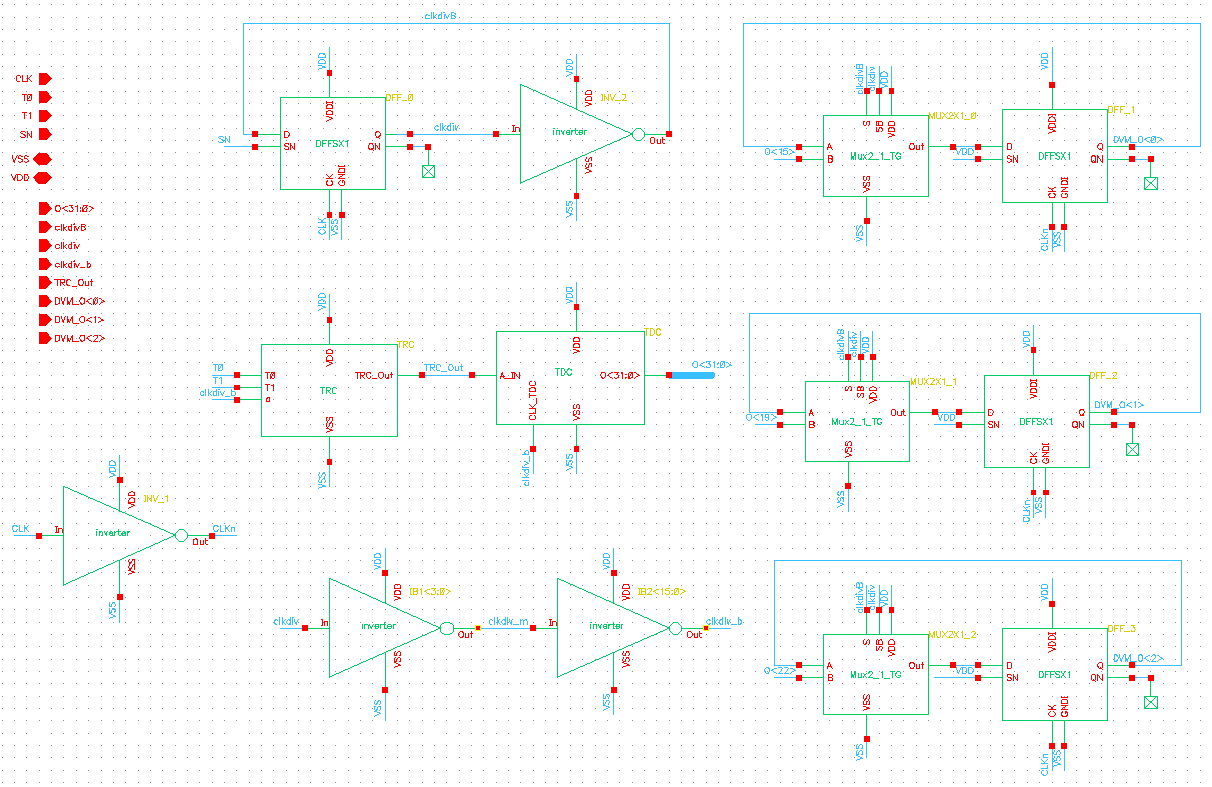
\includegraphics[width=0.52\textwidth]{extra_images/img_dvm_sch_v2_c.png} &
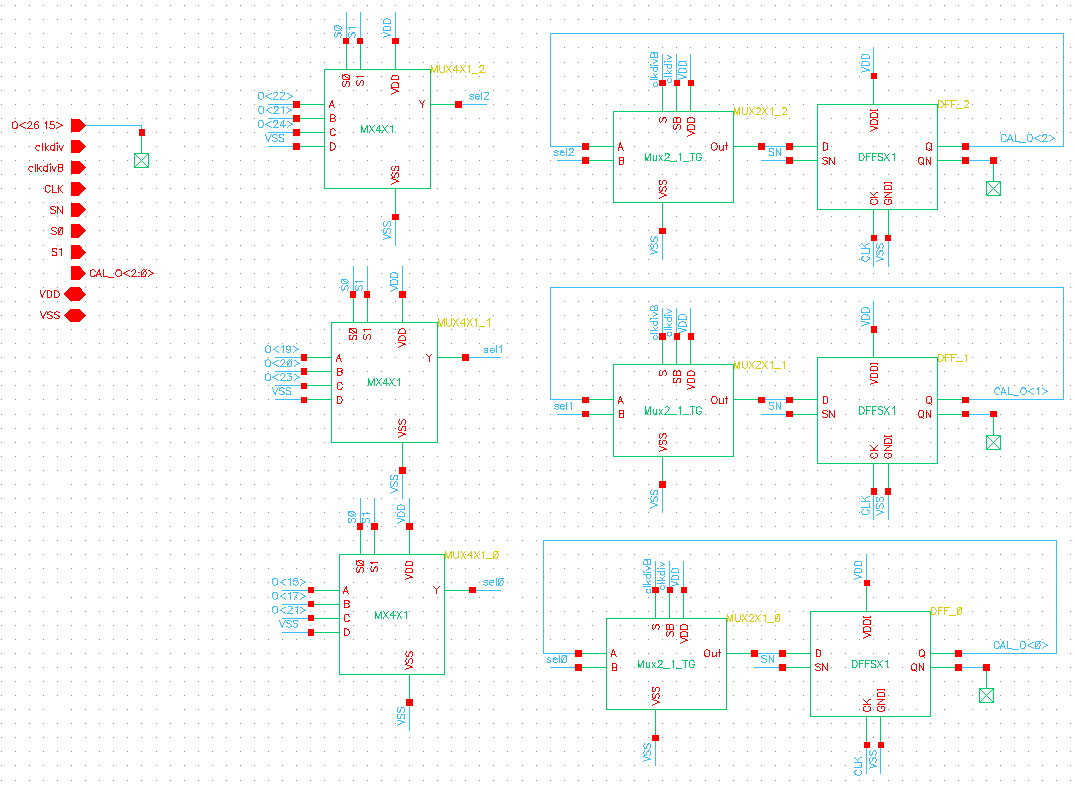
\includegraphics[width=0.46\textwidth]{extra_images/img_tapcal_sch_v2_c.png} \\[-2pt]
\footnotesize (a) DVM & \footnotesize (b) TAP\_CAL
\end{tabular}
\caption{Cadence schematics: (a) DVM top level; (b) TAP\_CAL.}
\label{fig:sch}
\end{figure*}

\section*{Appendix B: AI Interactions}
An AI assistant (Claude, Anthropic) was used in a chat interface throughout the project. It did not run any design tool; all schematics, layouts, extractions and simulations were done by the authors in Cadence, and every reported number comes from the authors' simulations. Table~\ref{tab:ai} lists the interactions by phase.

\begin{table}[!h]
\caption{AI Assistance by Project Phase}
\label{tab:ai}
\centering\footnotesize
\setlength{\tabcolsep}{3pt}
\begin{tabular}{p{0.28\columnwidth}p{0.66\columnwidth}}
\toprule
Phase & Assistance \\
\midrule
Proposal, Weeks 1--2 & Summaries of the reference papers, specification table, LaTeX formatting. \\
Schematic, Week 3 & Test-bench setup; ADE expressions for code, flags, latency and power; debugging decision-stage timing. \\
Layout, Week 4 & Interpreting Assura LVS reports (label opens, shorted pins, pin-swap artefact). \\
Post-layout and PVT & Diagnosis of the post-layout failure (clock buffer, 800~MHz, taps); corner and Monte Carlo plans; TAP\_CAL concept and tap tables. \\
Test-bench code & Verilog-A droop sources (single droop, droop train, droop matrix) and the debug-only tap monitor, written by the assistant and checked by the authors. \\
Figures & Python scripts that plot the exported simulation data; the hierarchy figure (Fig.~\ref{fig:hier}). \\
Report & Drafting and editing text. \\
\bottomrule
\end{tabular}
\end{table}



\end{document}
